\documentclass[10pt]{article}
\usepackage[margin=0.85in]{geometry}
\usepackage{amsmath, amssymb, amsthm, mathtools}
\usepackage{graphicx, booktabs, caption, xcolor, enumitem}
\usepackage[T1]{fontenc}\usepackage{lmodern}
\usepackage[hidelinks]{hyperref}
\captionsetup{font=small, labelfont=bf}
\setlength{\parskip}{3pt}\setlength{\parindent}{0pt}
\setlist{nosep, leftmargin=1.4em}
\newcommand{\cLtraj}{3.05}
\newcommand{\cLbox}{5.34}
\newcommand{\cmu}{1.17}
\newcommand{\cLtilde}{10.56}
\newcommand{\cetamax}{0.159}
\newcommand{\cNobs}{101}
\newcommand{\cnoiseslack}{4.9}
\newcommand{\cnoiseslackrule}{5.6}
\newcommand{\cynormmax}{2.34}
\newcommand{\cattractoroverone}{15}
\newcommand{\cpeakamp}{8.5}
\newcommand{\cpeaksens}{15.1}
\newcommand{\cperiod}{39.5}
\newcommand{\cmeanmu}{0.29}
\newcommand{\cweights}{3.54}
\newcommand{\cmuDglobal}{1.00}
\newcommand{\cfracDneg}{75}
\newcommand{\cmeanmuD}{0.077}
\newcommand{\cmulower}{-2.96}

\newcommand{\orig}[1]{\textcolor{black!60}{\textbf{Original.}} #1}
\newcommand{\prop}[1]{\textcolor{blue!60!black}{\textbf{Proposed.}} #1}
\newcommand{\gain}[1]{\textcolor{green!45!black}{\textbf{Why it is better.}} #1}
\newcommand{\norm}[1]{\lVert #1\rVert}
\newcommand{\dd}{\,\mathrm{d}}
\newtheorem*{lemA}{Lemma 1}
\title{\vspace{-1.6em}\textbf{R003 --- Sharper error bounds for multiple shooting with the same machinery}\\
\large Original bounds of the manuscript, the proposed replacements, and how much each change buys\\
\normalsize(\texttt{reports/2026-09-11-R003-tighter-error-bounds/})\\[3pt]\normalsize 11 September 2026}
\author{\vspace{-4.5em}}
\date{\vspace{-4.5em}}
\begin{document}
\maketitle
\vspace{-2.2em}

\paragraph{Summary.} The manuscript \emph{Sparse Optimization using Multi-Shooting and Guess Propagation} bounds everything by $e^{L t}$ with $L$ a Lipschitz constant of the right-hand side. On the FitzHugh--Nagumo (FHN) system the measured amplification of an initial-state error never exceeds $\cpeakamp$, while $e^{L t}$ reaches $10^{13}$ at $t=10$ (report R002, Figures~8--10). Four changes, each a one-line modification of an existing proof, close most of that gap:
\begin{enumerate}
\item replace the Lipschitz constant $L$ by the \emph{logarithmic norm} $\mu\le L$ (Lemmas 1, 2, Proposition 1, Theorem 1); on FHN this is $\cLtraj\to\cmu$ in the exponent, and $\mu$ is a \emph{global} constant for FHN whereas $L$ grows with the region;
\item remove the attractor-size factor $C^{(2)}_k=\max\norm{y_{i+1}}$ from Proposition~1, which makes its bound quadratic instead of linear in the small quantities (a factor of about $\cattractoroverone$ here);
\item state the noise terms in expectation instead of via $\norm{\eta}_{\max}$ (a factor $\cnoiseslack$ on this data set), and sum the per-datum exponentials as a geometric series instead of taking $e^{L\Delta T}$ for all of them;
\item as a trajectory-dependent refinement, integrate the local logarithmic norm over each window; in a diagonally weighted norm most FHN windows are then \emph{contracting} and the worst window has amplification $\le 8$ for every window length tested, which is the observed number.
\end{enumerate}
What cannot be fixed with Gr\"onwall-type arguments is also stated (\S\ref{sec:limits}). All numbers are recomputed from the R002 result files copied into \texttt{external\_data/}; the eight gates in \texttt{analysis/verify\_R003.py} all pass (\S\ref{sec:gates}). Table~\ref{tab:lemmas} and Figure~\ref{fig:1} carry the comparison.

\paragraph{Notation in one paragraph.} $\dot x=f(x;p)$, $x\in\mathbb R^d$, true parameter $p^\star$, flow $\varphi_f(t;p,x_0)$; data $y_i=x_i+\eta_i$ at times $t_i$, $i=0,\dots,N$, spacing $\Delta t$; shooting nodes $\tau_k$ with window length $\Delta T=\max_k(\tau_k-\tau_{k-1})$; $J_K(p)=\sum_k\sum_{t_i\in[\tau_{k-1},\tau_k]}\norm{\varphi_f(t_i-\tau_{k-1};p,y_{\tau_{k-1}})-y_i}^2$; $J_f=\partial f/\partial x$. $L=\sup\norm{J_f}_2$ is the Lipschitz constant in $x$, $\tilde L=\sup\norm{\partial f/\partial p}_2$ the one in $p$. The \emph{logarithmic norm} (one-sided Lipschitz constant, Dahlquist) is
\begin{equation}\label{eq:mu}
\mu:=\sup_x\lambda_{\max}\!\Big(\tfrac12\big(J_f(x)+J_f(x)^\top\big)\Big),\qquad\text{equivalently}\quad \langle f(x)-f(z),\,x-z\rangle\le\mu\norm{x-z}^2 .
\end{equation}
Always $-L\le\mu\le L$; unlike $L$, $\mu$ can be zero or negative. FHN constants measured in R002 along the true orbit: $L=\cLtraj$ ($\cLbox$ on the box $[-2.5,2.5]\times[-1,2]$), $\mu=\cmu$, $\tilde L=\cLtilde$, $\norm{\eta}_{\max}=\cetamax$, $N=\cNobs$, $d=2$.

\section{Lemma 1: sensitivity to the initial state}
\orig{} $\norm{\varphi_f(t;p,x_1)-\varphi_f(t;p,x_2)}\le e^{L t}\norm{x_1-x_2}$, proved from $\norm{\dot\delta}\le L\norm\delta$ for $\delta=\hat x_1-\hat x_2$.

\prop{} $\norm{\varphi_f(t;p,x_1)-\varphi_f(t;p,x_2)}\le e^{\mu t}\norm{x_1-x_2}$, and from below $\ge e^{\mu_- t}\norm{x_1-x_2}$ with $\mu_-=\inf_x\lambda_{\min}(\tfrac12(J_f+J_f^\top))\ge -L$. The proof differs from the original in one line: differentiate the \emph{square} of the norm instead of the norm,
\begin{equation}\label{eq:proof1}
\tfrac12\tfrac{\dd}{\dd t}\norm{\delta}^2=\big\langle\delta,\,f(\hat x_1;p)-f(\hat x_2;p)\big\rangle
=\Big\langle\delta,\Big(\textstyle\int_0^1 J_f(\hat x_2+s\delta)\dd s\Big)\delta\Big\rangle\le\mu\norm{\delta}^2 ,
\end{equation}
then $\tfrac{\dd}{\dd t}\norm\delta\le\mu\norm\delta$ and Gr\"onwall gives the claim. The middle equality is the mean-value form of $f(\hat x_1)-f(\hat x_2)$ and is exact. The original proof bounds $\langle\delta,\dot\delta\rangle$ by Cauchy--Schwarz, $\norm\delta\norm{\dot\delta}\le L\norm\delta^2$, which discards the sign information in the inner product; \eqref{eq:proof1} keeps it.

\gain{} Table~\ref{tab:lemmas} (left) and Figure~\ref{fig:1}(a). At the window lengths the paper actually uses ($\Delta T=1,2$) the proposed bound sits within a factor $1.1$--$1.5$ of the observed peak, where the original is off by a factor $7$--$65$; at $\Delta T=10$ the gap shrinks from $10^{12}$ to $10^{4}$. Two further points specific to FHN. First, $\mu$ is a \emph{global} constant: the FHN Jacobian is $\begin{psmallmatrix}1-v^2&-1\\0.08&-0.064\end{psmallmatrix}$, and $1-v^2\le1$ for every $v$, so $\mu=\cmu$ on all of $\mathbb R^2$ (attained at $v=0$), while $L$ grows like $v^2$ and is already $\cLbox$ on the R002 box. The proposed Lemma~1 therefore holds for perturbations of any size with the same constant; the original needs a neighbourhood. Second, the exponent is still positive, so the proposed bound still grows without limit while the true amplification turns around at $t\approx3$ (the orbit is attracting); \S\ref{sec:windows} and \S\ref{sec:limits} address this.

\begin{table}[t]\centering\small
\caption{Original versus proposed bounds on FHN, evaluated at $t=\Delta T$, against the largest value observed over the 24 R002 probes for $t\le\Delta T$ (Lemma~1: $x_2=x_1+10^{-3}u$, $u$ a random unit vector, at four orbit phases; Lemma~2: $p_2=p^\star+10^{-3}u$, $u\in\mathbb R^{20}$). All bounds hold on every probe (gates G4--G7). Source: \texttt{analysis/results/lemma1\_table.csv}, \texttt{lemma2\_table.csv}.}\label{tab:lemmas}
\begin{tabular}{r rrr rrr}
\toprule
& \multicolumn{3}{c}{Lemma 1: $\lVert\varphi(t;x_1)-\varphi(t;x_2)\rVert/\lVert x_1-x_2\rVert$} & \multicolumn{3}{c}{Lemma 2: $\lVert\varphi(t;p_1,x_0)-\varphi(t;p_2,x_0)\rVert/\lVert p_1-p_2\rVert$}\\
\cmidrule(lr){2-4}\cmidrule(lr){5-7}
$t=\Delta T$ & original $e^{L\Delta T}$ & proposed $e^{\mu\Delta T}$ & observed peak & original $\frac{\tilde L}{L}(e^{L\Delta T}-1)$ & proposed $\frac{\tilde L}{\mu}(e^{\mu\Delta T}-1)$ & observed peak\\
\midrule
1 & 21.1 & 3.23 & 2.93 & 69.8 & 20.1 & 3.7 \\
2 & 447 & 10.4 & 6.92 & $1.5\times10^{3}$ & 84.9 & 6.7 \\
5 & $4.2\times10^{6}$ & 349 & 8.48 & $1.5\times10^{7}$ & $3.1\times10^{3}$ & 12.0 \\
10 & $1.8\times10^{13}$ & $1.2\times10^{5}$ & 8.48 & $6.2\times10^{13}$ & $1.1\times10^{6}$ & 15.1 \\
\bottomrule
\end{tabular}

\end{table}

\section{Lemma 2: sensitivity to the parameters}
\orig{} $\norm{\varphi_f(t;p_1,x_0)-\varphi_f(t;p_2,x_0)}\le\frac{\tilde L}{L}\big(e^{Lt}-1\big)\norm{p_1-p_2}$.

\prop{} $\norm{\varphi_f(t;p_1,x_0)-\varphi_f(t;p_2,x_0)}\le\frac{\tilde L}{\mu}\big(e^{\mu t}-1\big)\norm{p_1-p_2}$, read as $\tilde L\,t\norm{p_1-p_2}$ when $\mu=0$ and as $\frac{\tilde L}{|\mu|}\big(1-e^{-|\mu|t}\big)\norm{p_1-p_2}\le\frac{\tilde L}{|\mu|}\norm{p_1-p_2}$ when $\mu<0$. Proof: split $\dot\delta=[f(\hat x_1;p_1)-f(\hat x_2;p_1)]+[f(\hat x_2;p_1)-f(\hat x_2;p_2)]$ exactly as in the manuscript, but take the inner product with $\delta$ first:
$\tfrac12\tfrac{\dd}{\dd t}\norm\delta^2\le\mu\norm\delta^2+\tilde L\norm\delta\norm{p_1-p_2}$, hence $\tfrac{\dd}{\dd t}\norm\delta\le\mu\norm\delta+\tilde L\norm{p_1-p_2}$, and the manuscript's integrating-factor step finishes it.

\gain{} Table~\ref{tab:lemmas} (right), Figure~\ref{fig:1}(b). Beyond the constant-factor gain, the proposed form is qualitatively right in a way the original cannot be: for a dissipative system ($\mu<0$) it \emph{saturates} at $\tilde L/|\mu|$, which is exactly the shape R002 Figure~9 shows (the observed sensitivity levels off at $\cpeaksens$). A Lipschitz constant is non-negative by definition, so $\frac{\tilde L}{L}(e^{Lt}-1)$ can never predict saturation. On FHN in the Euclidean norm $\mu=\cmu>0$, so saturation is not yet proved by this step alone; the weighted norm of \S\ref{sec:windows} gets closer.

\section{Proposition 1 and Theorem 1: cost change under node removal}
These two results compare the cost $J_K$ on a fine partition with the cost $\hat{\mathcal J}_K$ after the nodes indexed by $\mathcal I_R$ are removed. Three independent changes apply.

\textbf{(a) Substitute $\mu$ for $L$.} Both results use Lemmas~1 and~2 only through the factors $e^{L\Delta T_1}$, $e^{L\Delta T_2}$ and $\frac{\tilde L}{L}(e^{L\Delta T_2}-1)$; each becomes its $\mu$ version verbatim.

\textbf{(b) Remove the attractor-size constant.} \orig{} the proof writes the per-datum difference of squared residuals as $\norm{u-v}\,\norm{u+v-2y_{i+1}}$ with $u,v$ the two model predictions, then bounds the second factor by $2C^{(1)}_k+2C^{(2)}_k$ where $C^{(2)}_k=\max\norm{y_{i+1}}$ is the size of the data, $\cynormmax$ on FHN. \prop{} write $a=\norm{u-y_{i+1}}$, $b=\norm{v-y_{i+1}}$ (the two residuals) and use $a^2-b^2=(a-b)(a+b)$ with $|a-b|\le\norm{u-v}$ (reverse triangle inequality) and $a+b\le 2\max(a,b)$. Near $p^\star$ each residual is bounded by Lemmas~1--2 as $e^{\mu\Delta T_1}\norm{\eta}_{\max}+\norm{\eta}_{\max}+\frac{\tilde L}{\mu}(e^{\mu\Delta T_1}-1)\norm{p-p^\star}$, so the constant $C_{\max}$ in
\[
|\hat{\mathcal J}_K(p)-J_K(p)|\le 2|\mathcal I_R|\,C_{\max}\Big(e^{\mu(\Delta T_1+\Delta T_2)}\norm{\eta}_{\max}+e^{\mu\Delta T_1}\big[\tfrac{\tilde L}{\mu}(e^{\mu\Delta T_2}-1)\norm{p-p^\star}+\norm{\eta}_{\max}\big]\Big)
\]
is now $O(\norm\eta+\norm{p-p^\star})$ instead of $O(\norm y)$. \gain{} the right-hand side becomes \emph{quadratic} in the small quantities, as the left-hand side is (a difference of two squared residuals of size noise), instead of linear times the attractor radius; on FHN $\norm{y}_{\max}/\norm{\eta}_{\max}\approx\cattractoroverone$, so this is the largest constant-factor loss in Proposition~1 and it propagates unchanged into Theorem~1 through $C_{\max}$. It also makes the theorem's bound on $\norm{\hat p^{(K)}-p^{(K)}}$ scale like the noise, not like $\sqrt{\text{noise}\times\text{attractor size}}$.

\textbf{(c) Two free tightenings of the summation.} (i) The proofs apply $e^{L\Delta T}$ to every datum in a window, but datum $t_i$ only sees $e^{L(t_i-\tau_{k-1})}$; summing the geometric series over the $n_k$ data in a window replaces $n_k e^{2L\Delta T}$ by $\frac{e^{2L\Delta T}-1}{e^{2L\Delta t}-1}\approx\frac{e^{2L\Delta T}}{2L\Delta t}$, a saving of order $L\Delta T$ for $n_k=\Delta T/\Delta t$. (ii) Every $\norm{\eta_i}$ is replaced by $\norm{\eta}_{\max}$. Under the manuscript's own Gaussian model, $\mathbb E\norm{\eta_i}^2=d\sigma^2$ while $\norm{\eta}_{\max}^2\approx\sigma^2(d+2\log N)$, a factor $1+2\log N/d$ ($\cnoiseslackrule$ for $N=\cNobs$, $d=2$; measured $\cnoiseslack$ on the R002 data set). Moreover the node noise $\eta_{\tau_{k-1}}$ and the datum noise $\eta_i$ are independent for $t_i\ne\tau_{k-1}$, so the cross term in $(e^{L\Delta T}\norm{\eta_{\tau_{k-1}}}+\norm{\eta_i})^2$ vanishes in expectation, saving a further factor up to $2$. A bound on $\mathbb E\,J_K(p^\star)$ is therefore both tighter and the natural object for the strong-convexity step that follows it. A typo to fix while there: equation (JK11) in the proof has $e^{2L(\Delta T_1+\Delta T_2)}$ while the statement of Proposition~1 has $e^{L(\Delta T_1+\Delta T_2)}$.

\begin{figure}[t]\centering
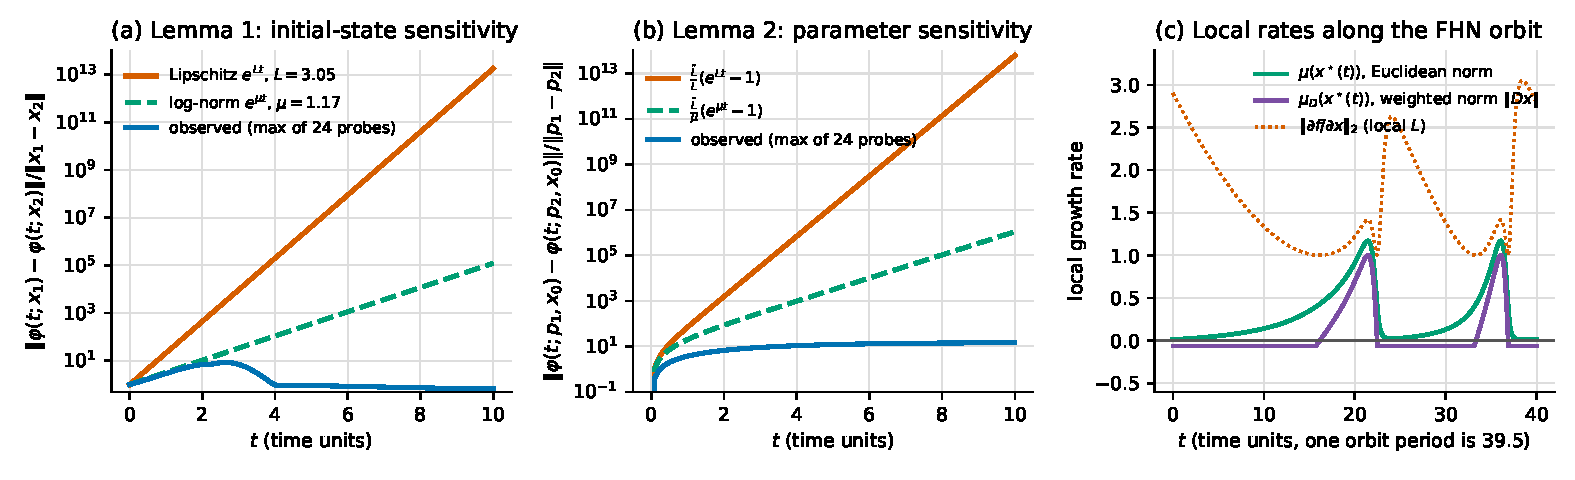
\includegraphics[width=\textwidth]{figures/fig01_bounds.pdf}
\caption{(a) Lemma~1 and (b) Lemma~2 on FHN: the original Lipschitz bound (solid vermilion), the proposed log-norm bound (dashed green), and the largest observed ratio over the 24 R002 probes at each $t$ (blue). Both bounds hold at every probe; the proposed one is $10^{8}$ closer at $t=10$ but still grows, while the observation turns around because the orbit is attracting. (c) The local rates along one FHN period: the local Lipschitz constant $\norm{\partial f/\partial x}_2$ (dotted) is never below $1$; the Euclidean log norm $\mu(x^\star(t))$ (green) is near $0$ on the slow branches and peaks at $\cmu$ only during the two fast jumps; in the weighted norm $\norm{Dx}$, $D=\mathrm{diag}(1,\cweights)$, the local log norm $\mu_D$ (purple) is \emph{negative} ($-0.064$) for $\cfracDneg\,\%$ of the period. Data: \texttt{analysis/results/envelopes.csv}, \texttt{local\_lognorm.csv}, \texttt{local\_lognorm\_D.csv}.}\label{fig:1}
\end{figure}

\section{Refinement: per-window exponents and a weighted norm}\label{sec:windows}
\orig{} one constant $e^{L\Delta T}$ (or $e^{\mu\Delta T}$ after \S1) for every window.

\prop{} The mean-value form in \eqref{eq:proof1} holds pointwise in time, so with $\mu(t):=\lambda_{\max}\big(\tfrac12(A(t)+A(t)^\top)\big)$, $A(t)=\int_0^1 J_f(\hat x_2(t)+s\delta(t))\dd s$, the same argument gives the exact bound $\norm{\delta(t)}\le\exp\!\big(\int_0^t\mu(s)\dd s\big)\norm{\delta(0)}$. Per window this is $e^{\Lambda_k}$ with $\Lambda_k=\int_{\tau_{k-1}}^{\tau_k}\mu(s)\dd s$, and Lemmas~1--2, Proposition~1 and Theorem~1 go through with $e^{\mu\Delta T}$ replaced by $\max_k e^{\Lambda_k}$. For small perturbations $\mu(s)$ is the log norm of $J_f$ along the reference orbit (first-order in $\norm{\delta}$; for a rigorous statement take the supremum over the segment between the two trajectories). The same proof also runs in any weighted norm $\norm{x}_D=\norm{Dx}$ with $\mu_D$ the log norm of $DJ_fD^{-1}$, and returns to the Euclidean norm at the cost of the condition number $\kappa(D)$. For FHN the choice $D=\mathrm{diag}(1,s)$, $s=\sqrt{|J_{12}|/|J_{21}|}=\cweights$, makes the off-diagonals of $DJ_fD^{-1}$ equal and opposite, so its symmetric part is diagonal and $\mu_D(x)=\max(1-v^2,\,-0.064)$: negative whenever $|v|>1$, i.e.\ on both slow branches, with global supremum $\cmuDglobal$.

\gain{} Table~\ref{tab:windows}. In the weighted norm the worst window over the whole record has amplification $\le 8.04$ for \emph{every} window length tested (multiply by $\kappa(D)=\cweights$ to convert to a Euclidean statement), against the observed peak $\cpeakamp$ and the a-priori $e^{\mu\Delta T}$ of $1.2\times10^5$ at $\Delta T=10$; the median window contracts. The mean log norm over the record is $\cmeanmu$ (Euclidean) and $\cmeanmuD$ (weighted), so over a period the orbit is nearly neutral, as it must be (the phase direction has Floquet exponent zero). Two consequences for the paper. First, this is the quantitative version of ``the restart at each node resets the error'': the per-window exponents are what the schematic R002 Figure~7 should be drawn with. Second, it gives a node-placement rule sharper than the one after Proposition~1 (``remove nodes with small $\eta_{\tau_k}$ and small $\Delta T_2$''): place and keep nodes just before the fast jumps, where $\int\mu$ accumulates, and remove them freely on the slow branches, where every window is contracting. The price is that $\Lambda_k$ is evaluated along the fitted orbit, so the bound is a posteriori rather than a closed-form constant.

\begin{table}[t]\centering\small
\caption{Per-window amplification along the true FHN orbit ($\Delta t=1$, $\cNobs$ data, windows aligned to $t_0$). ``Worst'' and ``median'' are $\max_k$ and median$_k$ of $e^{\Lambda_k}$ over the windows of that length; ``contracting'' is the share of windows with $\Lambda^D_k<0$. Weighted-norm values convert to Euclidean statements by a factor at most $\kappa(D)=\cweights$. Source: \texttt{analysis/results/window\_exponents.csv}, \texttt{window\_exponents\_D.csv}.}\label{tab:windows}
\begin{tabular}{r r r rr rr r}
\toprule
& & a priori & \multicolumn{2}{c}{per-window $e^{\Lambda_k}$, Euclidean} & \multicolumn{3}{c}{per-window $e^{\Lambda^D_k}$, weighted norm}\\
\cmidrule(lr){4-5}\cmidrule(lr){6-8}
$\Delta T$ & windows & $e^{\mu\Delta T}$ & worst & median & worst & median & contracting windows\\
\midrule
1 & 100 & 3.23 & 3.10 & 1.16 & 2.60 & 0.94 & 74\,\% \\
2 & 50 & 10.4 & 8.56 & 1.41 & 5.89 & 0.88 & 70\,\% \\
5 & 20 & 349 & 34.78 & 3.75 & 8.04 & 0.73 & 55\,\% \\
10 & 10 & $1.2\times10^{5}$ & 138.79 & 29.25 & 5.89 & 3.20 & 30\,\% \\
\bottomrule
\end{tabular}

\end{table}

\section{What this machinery cannot do}\label{sec:limits}
Any a-priori bound valid for every $f$ with a given $L$ (or $\mu$) is attained by the linear system $\dot x=Lx$ (or $\dot x=\mu x$) and is therefore exponential; no rearrangement of a Gr\"onwall argument removes the exponential. The observed plateau at $\cpeakamp$ in Figure~\ref{fig:1}(a) is a property of the FHN attractor, not of any Lipschitz-type constant. Proving it needs one of: a contraction metric with $\mu_P<0$ everywhere, which does not exist on a limit cycle because the phase direction is neutral (\S\ref{sec:windows} gets $\mu_D<0$ on $\cfracDneg\,\%$ of the period, not all of it); a Lyapunov function for the attractor, giving boundedness of perturbations but not a rate; or a Floquet analysis of the variational equation about the periodic orbit, which bounds the transverse contraction rate but requires the orbit to be known. All three are more machinery than the manuscript uses. The honest summary is: \S1--\S3 make the constants of the right kind (they can saturate and are global for FHN) at no cost in rigour or length; \S\ref{sec:windows} makes them quantitatively close along the actual orbit at the cost of being trajectory-dependent; the remaining gap is intrinsic to worst-case analysis.

\section{Gates and reproduction}\label{sec:gates}
\texttt{analysis/verify\_R003.py} writes \texttt{analysis/results/gates\_summary.json}. G1: the seven input files match the SHA-256 hashes in \texttt{INPUTS.md}. G2: $L$, $\tilde L$, $\mu$ recomputed from the FHN library file agree with R002's \texttt{concept\_meta.json} to $10^{-3}$ relative, and $\mu$ recomputed on the R002 box equals the analytic global value $\lambda_{\max}$ at $v=0$ to $10^{-6}$. G3: $\mu\le L$ and the weighted-norm supremum $\mu_D=1$ to $10^{-9}$. G4/G5: the original and proposed Lemma~1 upper bounds hold at all $24\times101$ probe points (and the lower bounds $e^{-Lt}$, $e^{\mu_-t}$ with $\mu_-=\cmulower$). G6/G7: same for Lemma~2. G8: every number quoted in this text (Table~\ref{tab:lemmas}, Table~\ref{tab:windows}, the constants macros) is regenerated by \texttt{make\_tables.py} from \texttt{results/} and matches the committed \texttt{tables/*.tex} byte for byte. Outcome: \textbf{8/8 pass}. Regenerate with \texttt{compute\_R003.py}, \texttt{make\_tables.py}, \texttt{figures/make\_figures.py}, \texttt{verify\_R003.py}, then \texttt{pdflatex} twice (see \texttt{REPRODUCE.md}).
\end{document}
